\section{Conception}

\begin{frame}
\frametitle{Réseau de communication}
\begin{center}
\begin{figure}
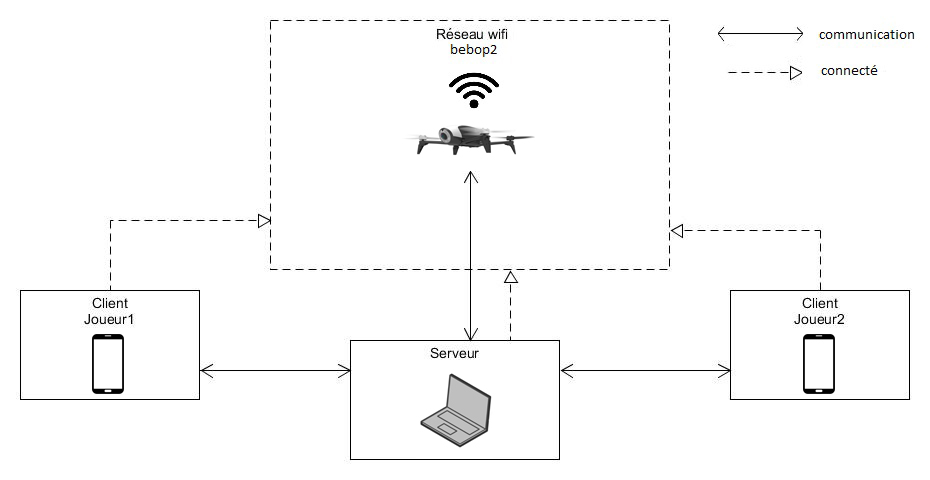
\includegraphics[scale=0.45]{images/architecture.jpg}
\end{figure}
\end{center}
\end{frame}

\begin{frame}
\frametitle{Jeu mobile}
\begin{multicols}{2} 
\begin{itemize}
\item Jeu de rythme
\item Prototype du client sous forme d'une application \android{}
\item 4 zones actives
\item Attente des joueurs dans un salon
\end{itemize} 
\columnbreak 
\begin{figure}
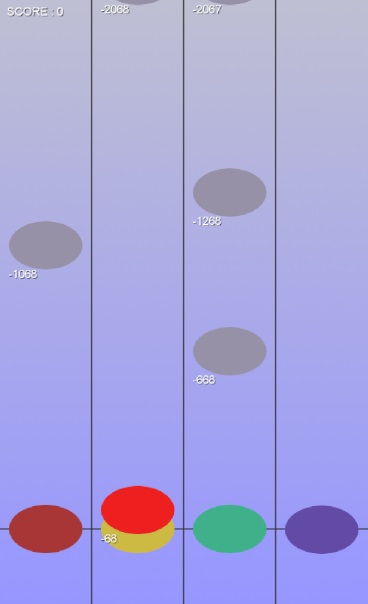
\includegraphics[scale=0.4]{images/jeu3.jpg}
\end{figure}
\end{multicols}
\end{frame}

\begin{frame}
\frametitle{Serveur et protocole de communication}
\begin{center}
\begin{itemize}
\item Protocole de communication textuel
\begin{enumerate}
\item Connexion 
\item Initialisation et lancement de la partie
\item Envoi périodique des scores
\end{enumerate}
\item Protocole UDP vs TCP
\end{itemize}
\begin{figure}
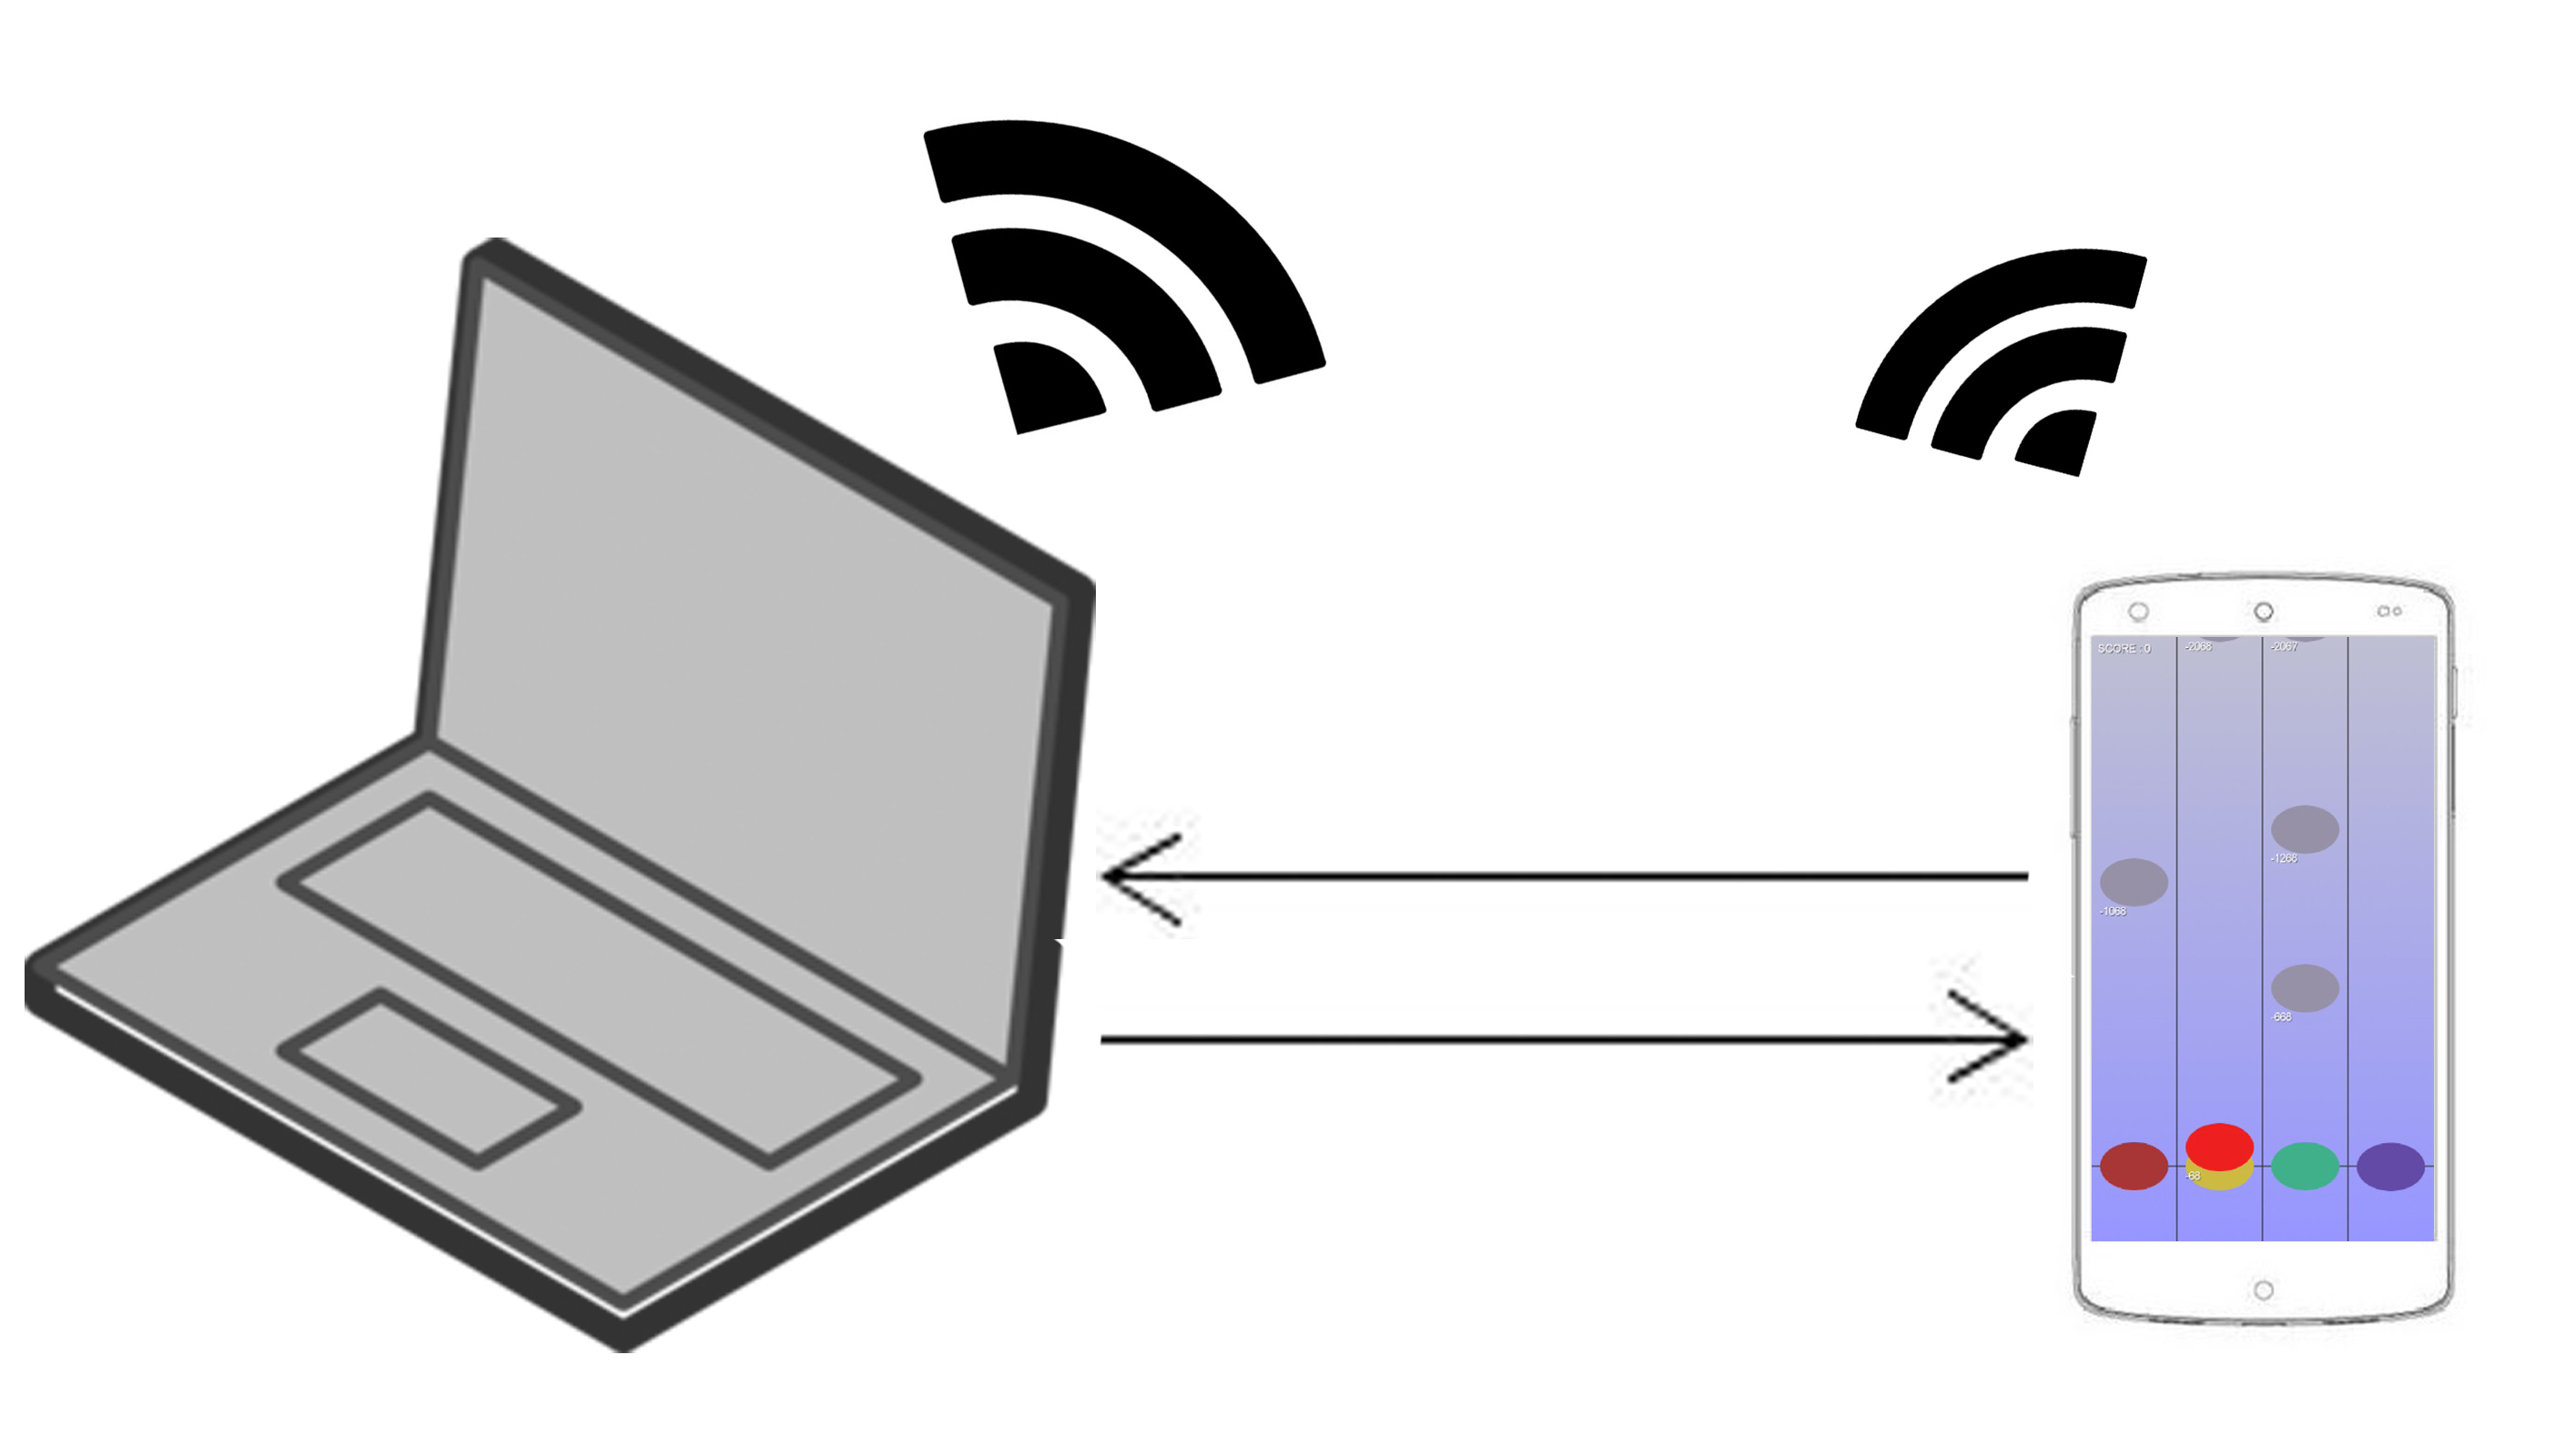
\includegraphics[scale=0.05]{images/client_serveur.jpg}
\end{figure}
\end{center}
\end{frame}

\begin{frame}
\frametitle{Drone et ARSDK}
\begin{center}
\begin{itemize}
\item Analyse et exploitation de la SDK (ARSDK Parrot)
\item Utilisation de l'API C du SDK
\item Mouvements opérationnels
\end{itemize}
\begin{exampleblock}{Exemples de primitives}
{\tiny
\verb!//Décollage! \newline
\verb!deviceController->aRDrone3->sendPilotingTakeOff(deviceController->aRDrone3);! \newline
\verb!//Prise de photo! \newline
\verb!deviceController->aRDrone3->sendMediaRecordPicture(deviceController->aRDrone3, 0);! \newline
\verb!//Angle du drone! \newline
\verb!deviceController->aRDrone3->setPilotingPCMDPitch(deviceController->aRDrone3, 50);!}
\end{exampleblock}
\end{center}
\end{frame}

\begin{frame}
\frametitle{Limitations et difficultés rencontrées}
\begin{center}
\begin{itemize}
\item Conditions de tests délicates
\begin{itemize}
\item Disponibilité du drone
\item Sécurité
\end{itemize}
\item Gestion propre de la position du drone complexe
\begin{itemize}
\item Facteurs extérieurs
\item Limites matérielles
\end{itemize}
\end{itemize}
\end{center}
\end{frame}